De meeste datacenters zijn uitgerust met 19\inch-kasten waarin 19\inch-servers hangen. De 19\inch-maat staat voor de breedte van de server. De hoogte van een serverkast wordt uitgedrukt in het aantal U. Een normale server, de zogenaamde pizza-doos, is 1U hoog. Harddisks liggen dan plat in de server. Zwaardere servers met meer harddisks hebben de harddisks vaak rechtop op hun zijkant staan die hot-swappable uit de voorkant van de server getrokken kunnen worden. Deze servers zijn 2U hoog.

\begin{figure}[H]
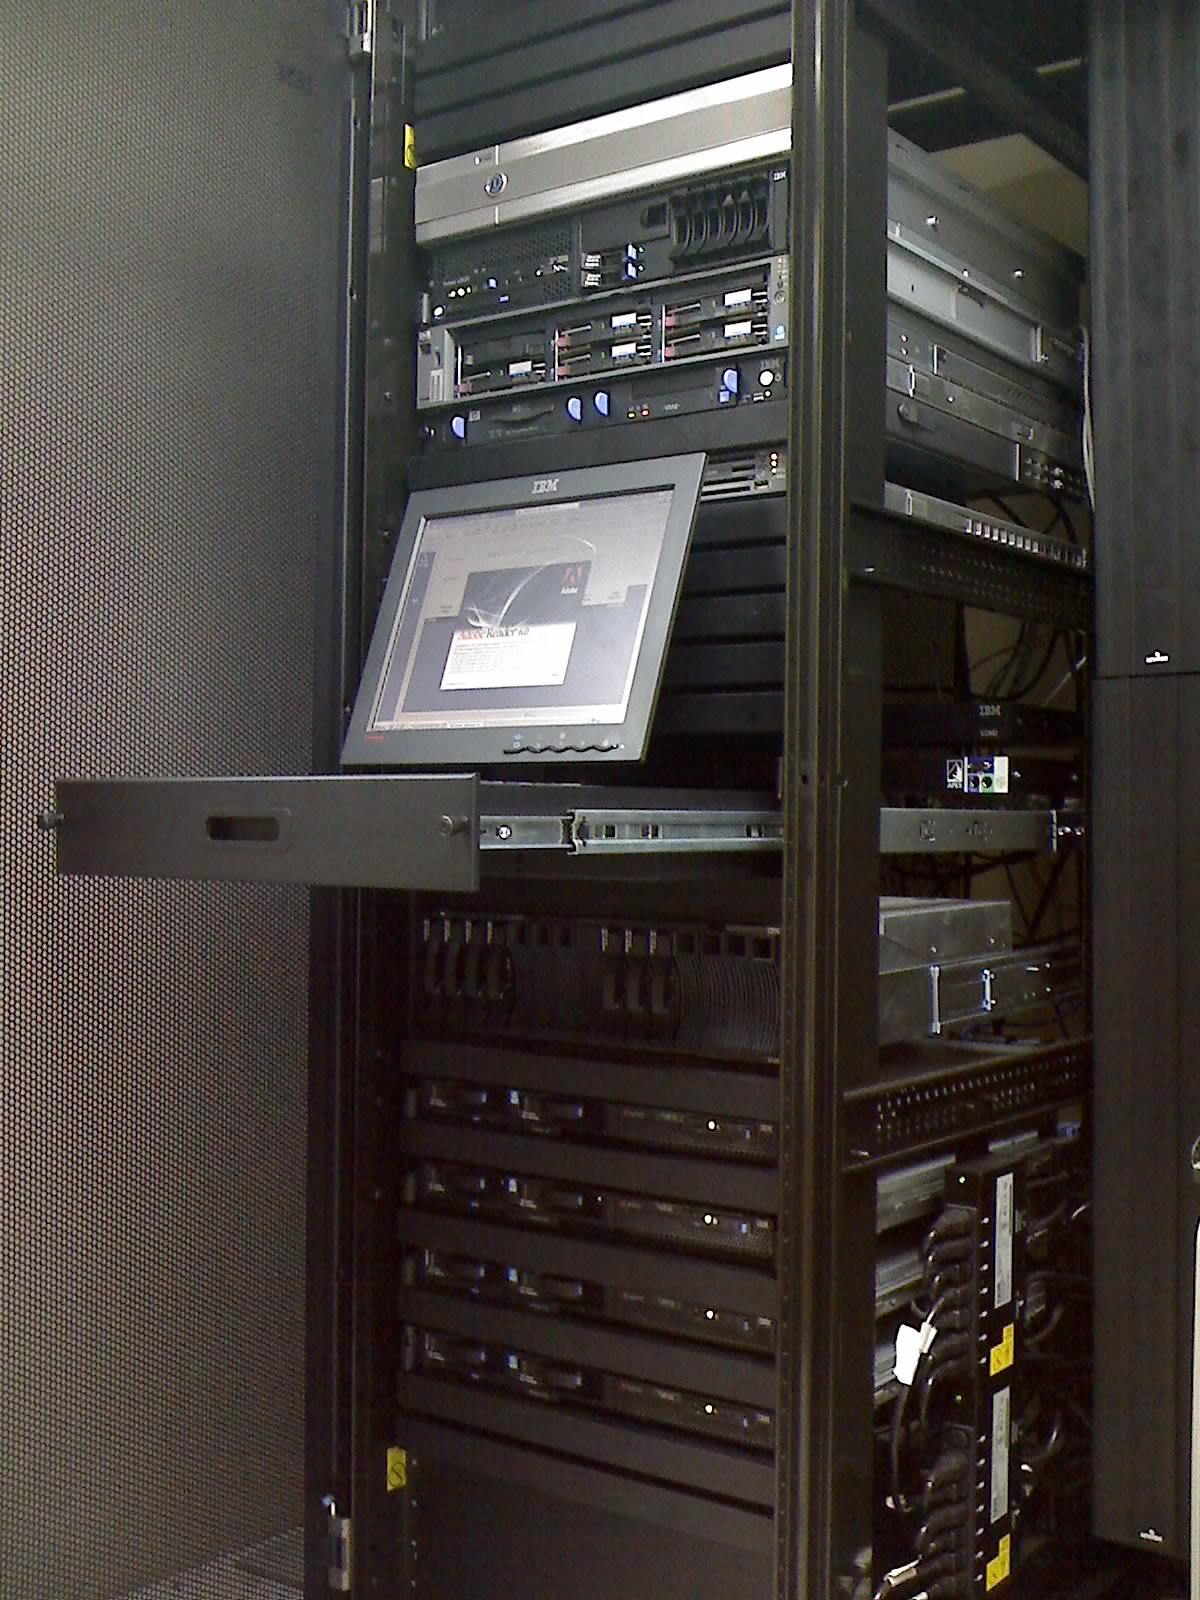
\includegraphics[width=0.75\linewidth]{Wiki_Rack001.jpg}
\caption Foto van Jfreyre afkomstig van \url{https://commons.wikimedia.org/wiki/File:Rack001.jpg}
\centering
\end{figure}

Om hogere dichtheden te bereiken wordt er gebruik gemaakt van blade servers\index{Blade servers}. Bij blade servers zitten er meedere servers (blades) in \'e\'en fysieke behuizing (19\inch-kast). De servers delen een backplane, de voeding(en) en de behuizing waardoor er effectief meer servers passen op dezelfde oppervlakte. Een nadeel van blades is wel dat de warmte ontwikkeling ook veel meer geconcentreerd wordt en dat kan leiden tot zogenaamde hotspots, wat slecht is voor de koeling.
